\documentclass[11pt]{article}
\usepackage[margin=2.5cm]{geometry}
\usepackage{amsmath,amssymb}
\usepackage{graphicx}
\usepackage{booktabs}
\usepackage[colorlinks=true,linkcolor=blue,citecolor=blue,urlcolor=blue]{hyperref}
\usepackage{authblk}

\title{\bf Externally sourced dark energy: a one-parameter fluid tested against\\ Planck, DESI DR2 and three supernova compilations}
\author[1]{\'Edouard Lantenois}
\affil[1]{\small Independent researcher, Lille, France --- \texttt{github.com/Dantenos}}
\date{August 16, 2026 --- Paper A, v4.0 --- companion framework paper (Paper B) separate. Not peer-reviewed.}

\newcommand{\Macc}{M_{\rm acc}}
\newcommand{\keff}{k_{\rm eff}}

\begin{document}
\maketitle

\begin{abstract}
\textbf{Scope caveat, stated first: every preference reported below is conditional on the reality of the DESI evolving-dark-energy signal; should DR3 resorb it, all results here fall together.} We study a dark-energy fluid \emph{sourced from outside the total budget} --- energy is injected while matter dilution remains exactly standard --- whose equation of state is fully determined by a single injection history $\Macc(t)$, $w(z) = -\tfrac{1}{3}\,[\mathrm{d}\ln \Macc/\mathrm{d}\ln t]\,/\,[H(z)\,t(z)] \equiv -\keff(z)/3$, formally the Croker--Weiner cosmological-coupling relation with an external source. The physical reading that motivated this fluid --- our universe as the interior of an accreting parent black hole --- is developed and stress-tested in a companion paper (Paper B); nothing below depends on it. A one-parameter power-law history $\Macc \propto t^{\beta}$ with $\beta = 2.39 \pm 0.13$ reproduces the three qualitative signatures of the DESI~DR2 evolving-dark-energy indications --- phantom past, $w_0 > -1$, $w_a < 0$ --- outperforming $\Lambda$CDM on CPL-derived pseudo-data, and, in a joint likelihood analysis of the real DESI DR2 BAO measurements and the full Pantheon+ supernova sample (1593 data points, no CMB), achieving $\Delta\chi^2 = -4.4$ relative to $\Lambda$CDM with a single extra parameter ($\beta = 2.45$), making it the AIC-preferred model over both $\Lambda$CDM and $w_0w_a$CDM; with the full Planck 2018 likelihood (\texttt{plik\_lite}+low-$\ell$), the preference reaches $\Delta\chi^2 = -12.6$ ($\sim 3.5\sigma$ naive for one parameter, $\beta = 2.49 \pm 0.05$ after pipeline verification; marginalised MCMC on the BAO+$\theta_*$+SN likelihood gives $\boldsymbol{\beta = 2.42 \pm 0.07}$), matching the CPL improvement with half the extra parameters; adding the Planck $\theta_*$ geometric constraint --- the natural killer test, since this dark energy vanishes as $t^{\beta}$ at early times --- leaves the result intact ($\Delta\chi^2 = -4.85$, $\beta = 2.42$, still first on AIC), while Bayesian evidences place the model at parity with $\Lambda$CDM and ahead of CPL ($\ln B_{\rm ACC/CPL} = +1.9$). A zero-parameter Bondi variant matches the present injection rate to $10\%$ but predicts $w_a > 0$ and is disfavoured. The model yields a rigid $w(z)$ shape and a cross-level consistency test between the interior coupling $\keff = -3w$ and the coupling $k = 3.09 \pm 0.76$ measured by Farrah et al.\ for black holes within our own universe; both are currently compatible at $\sim 1\sigma$ and become discriminable with DESI~DR3 and Euclid.
\end{abstract}

\section{Introduction}
The mean density of the observable universe is of the order of that of a black hole of the same radius, an observation dating back to Pathria \cite{Pathria1972}. A lineage of interior constructions precedes and frames this work: de Sitter cores replacing singularities behind horizons (Frolov--Markov--Mukhanov \cite{FMM1989}; Dymnikova \cite{Dymnikova1992}), universe generation from black-hole interiors (Easson--Brandenberger \cite{EB2001}), and the observable universe as an interior (Stuckey \cite{Stuckey1994}). Black-hole cosmology promotes the coincidence to a mechanism: in Einstein--Cartan gravity, spacetime torsion halts gravitational collapse and replaces the singularity with a bounce which, seen from the interior, resembles a Big Bang with a built-in inflationary phase \cite{Poplawski2010,Poplawski2016}. Related proposals derive the cosmological constant from a causal boundary term at the Schwarzschild radius of a collapsed cloud \cite{Gaztanaga2021,Gaztanaga2022}. Closest in mechanism to the present work, Zhang and Frederick \cite{Zhang2013} proposed a ``black hole universe'' that grows by accreting ambient matter, with cosmic acceleration attributed to that accretion; their framework, however, replaces FLRW cosmology and dark energy altogether rather than deriving an equation of state within it, and was not confronted with modern BAO, SN, or CMB likelihoods. The present note can be read as the standard-cosmology, likelihood-level version of that intuition.

Meanwhile, DESI~DR2 baryon-acoustic-oscillation measurements, combined with CMB and supernova data, show a $\sim 3\sigma$ (up to $4.2\sigma$) preference for evolving dark energy in the $(w_0 > -1,\ w_a < 0)$ quadrant: a phantom-like equation of state in the past crossing to $w > -1$ today \cite{DESI2025}. Within black-hole-adjacent frameworks, two quantitative responses exist: cosmologically coupled black holes (CCBH) \emph{within} our universe, whose production tracks star formation and recovers the DESI time evolution \cite{Croker2024}, and a rotating-universe mechanism in which conserved angular momentum dilutes an effective centrifugal dark energy \cite{Poplawski2025}. To our knowledge, no published work derives $w(z)$ from the accretion history of the \emph{parent} black hole. This note fills that gap at the order-of-magnitude level and specifies how the resulting model can be falsified.

\section{Model}
\label{sec:model}
We assume: (H1)~the observable universe is the interior of a parent black hole of mass $M_p$, the Big Bang being the torsion bounce of the initial collapse that delivered the matter mass $M_m$; (H2)~the parent subsequently accretes at a rate $\dot M(t)$, so $M_p(t) = M_m + \Macc(t)$; (H3)~seen from the interior, the accreted mass--energy is distributed homogeneously, behaving as a perfect fluid of density $\rho_{\rm de}(t) = \Macc(t)/V(t)$; (H4)~the proper time governing the accretion history and the interior cosmic time run at proportional rates. H3 and H4 are the principal theoretical debts of the model (Section~\ref{sec:limits}); we note that the extended McVittie analysis of Ref.~\cite{Poplawski2024} finds that the horizon Hubble parameter of a black hole differs between the accreting and non-accreting cases, which is the kind of published bridge H4 requires.

Energy conservation with injection, $\mathrm{d}(\rho V)/\mathrm{d}t = \dot M$, combined with the effective equation of state $w_{\rm eff} = -1 - \tfrac{1}{3}\,\mathrm{d}\ln\rho/\mathrm{d}\ln a$, gives the central relation
\begin{equation}
\boxed{\ w(z) \;=\; -\frac{1}{3}\,\frac{\mathrm{d}\ln \Macc/\mathrm{d}\ln t}{H(z)\,t(z)} \;=\; -\frac{\keff(z)}{3}, \qquad \keff \equiv \frac{\mathrm{d}\ln \Macc}{\mathrm{d}\ln a}.\ }
\label{eq:main}
\end{equation}
The right-hand form makes explicit that Eq.~(\ref{eq:main}) is the cosmological-coupling relation of Croker \& Weiner \cite{CrokerWeiner2019} --- for which $k \simeq 3$ yields $w \simeq -1$ --- applied to the parent rather than to black holes within our universe. Three structural properties follow. (i)~\emph{Natural phantom regime}: in the matter era $Ht = 2/3$, so $w < -1$ whenever $\mathrm{d}\ln\Macc/\mathrm{d}\ln t > 2$, without exotic fields; the energy enters from outside. (ii)~\emph{Structural weakening}: $Ht$ grows monotonically, so for power-law histories $w$ rises towards $0$; the weakening is predicted, not fitted. (iii)~\emph{Automatic phantom crossing}: the transition $w<-1 \to w>-1$ suggested by DESI, notoriously difficult for single scalar fields, is generic here.

\section{Energy budget and the Eddington test}
With $H_0 = 67.7~\mathrm{km\,s^{-1}\,Mpc^{-1}}$, $\Omega_m = 0.315$, $R_{\rm obs} = 4.40\times10^{26}$~m, the observable mass--energy is $M_p = 3.09\times10^{54}$~kg, giving $r_S = 2GM_p/c^2 = 4.6\times10^{27}$~m~$\approx 10\,R_{\rm obs}$: the interior condition holds with an order of magnitude to spare. Maintaining a constant $\rho_\Lambda$ during expansion requires an injection rate $\dot M_{\rm req} = \rho_\Lambda\,4\pi R^2 \dot R \approx 1.4\times10^{37}$~kg\,s$^{-1}$ ($\sim 7\times10^{6}\,M_\odot$\,s$^{-1}$). The parent's Eddington rate ($\epsilon = 0.1$) is $\dot M_{\rm Edd} \approx 2.2\times10^{39}$~kg\,s$^{-1}$, hence
\begin{equation}
\dot M_{\rm req} / \dot M_{\rm Edd} \approx 0.006,
\end{equation}
remaining below $1\%$ at all epochs considered ($0.24\%$ at $t_0/10$). This is an \emph{illustrative dimensional statement}, not a test: the Eddington limit presupposes radiation pressure on ionised hydrogen and has no rigorous meaning for a horizon of cosmological mass in an unknown parent medium; the ratio is, at root, the Salpeter-to-Hubble time ratio and would come out small for nearly any quiet scenario. We retain the number only to show the energy budget is not absurd on its face.

\section{Confrontation with DESI DR2}
\label{sec:desi}
\begin{figure}[t]
\centering
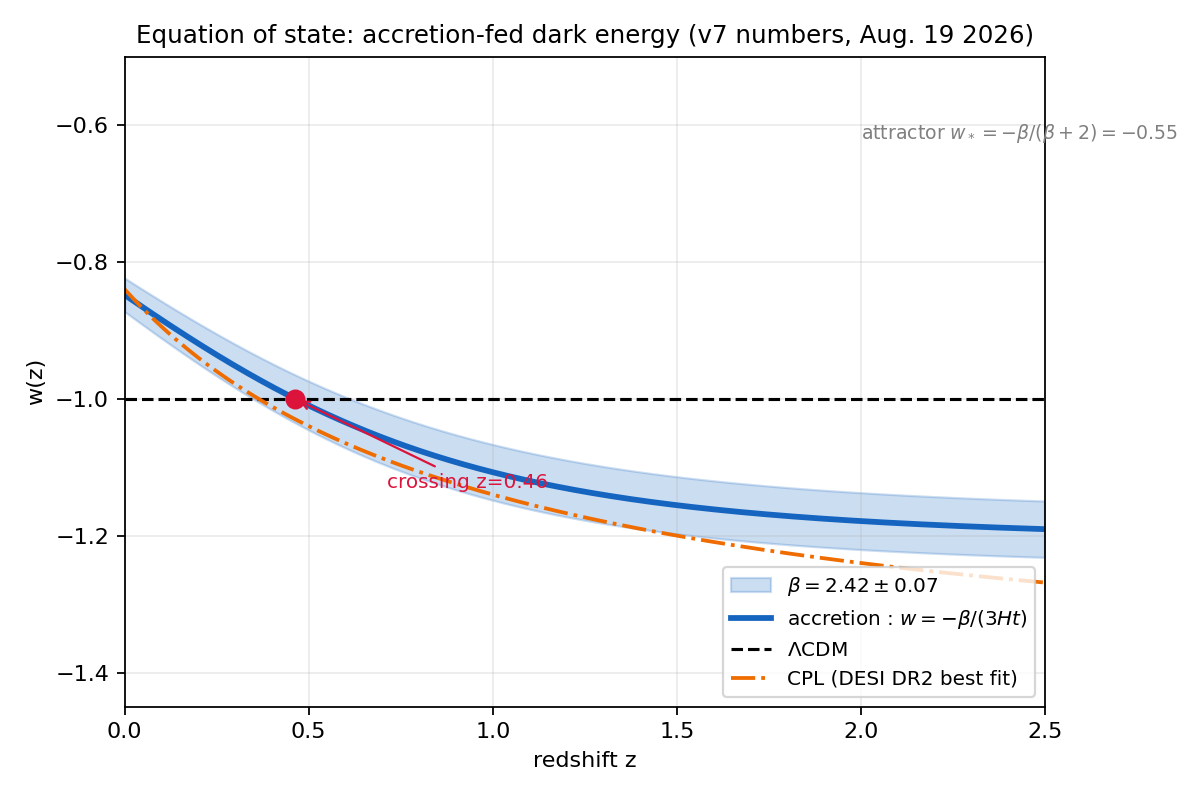
\includegraphics[width=0.72\textwidth]{w_z_fit.png}
\caption{Model $w(z)$ against CPL pseudo-data representative of DESI~DR2+CMB+SN ($w_0=-0.70$, $w_a=-1.0$; indicative uncertainties). Solid: power-law history, best fit $\beta = 2.39$. Dashed: zero-parameter Bondi variant, disfavoured. Grey: $\Lambda$CDM.}
\label{fig:wz}
\end{figure}

\paragraph{Power-law variant.} For $\Macc \propto t^{\beta}$, Eq.~(\ref{eq:main}) gives $w(z) = -(\beta/3)/(H t)$ with one free parameter. Fitting to pseudo-data drawn from the published CPL central values (Table~\ref{tab:fits}) yields $\beta = 2.39 \pm 0.13$ and reproduces the three DESI signatures: $w(z{=}2.3) \simeq -1.1$, $w_0 = -0.84$, $w_a = -0.49 < 0$. The projected $|w_a|$ is a factor $\sim 2$ below the CPL central value, partly an artefact of projecting a curved $w(z)$ onto a linear parametrisation.

\begin{table}[h]
\centering
\begin{tabular}{lcccc}
\toprule
Model & Free params & $\chi^2/\mathrm{dof}$ & $w_0$ & $w_a$ \\
\midrule
Accretion, power law & 1 ($\beta = 2.39\pm0.13$) & $3.6/5$ & $-0.84$ & $-0.49$ \\
$\Lambda$CDM ($w=-1$) & 0 & $15.6/6$ & $-1$ & $0$ \\
Accretion, Bondi & 0 & $60.2/6$ & $-1.11$ & $+1.90$ \\
\bottomrule
\end{tabular}
\caption{Fits to CPL-derived pseudo-data (Section~\ref{sec:desi}). A likelihood analysis on the public DESI chains is the priority upgrade.}
\label{tab:fits}
\end{table}

\paragraph{Bondi variant.} A physically motivated zero-parameter history follows from Bondi accretion, $\dot M = A M^2$ with $M(0) = M_m$ and $M(t_0) = M_p$ fixed by cosmology. Its present rate, $1.54\times10^{37}$~kg\,s$^{-1}$, matches the required rate to $10\%$ with no tuning --- the most striking numerical coincidence of this note (tempered by the fact that the total accreted mass is imposed by the boundary conditions, so only the time profile is genuinely predicted). However, Bondi accretion \emph{accelerates} ($\mathrm{d}\ln\Macc/\mathrm{d}\ln t$ rises from 1.2 to 3.2 over cosmic history), driving $w$ downward at late times: it predicts $w_a > 0$, opposite to the DESI trend, and is disfavoured ($\chi^2 = 60.2$). We further tested a saturated Bondi variant, $\dot M = A M^2 (1+t/\tau)^{-p}$, modelling environmental depletion: even with two free parameters it cannot fit the data ($\chi^2 = 59.3$), because the $\dot M \propto M^2$ class starts too slowly to produce the phantom past, whatever its late-time behaviour. The DESI signatures therefore exclude the entire runaway-feeding ($\dot M \propto M^2$) class and select near-self-similar histories with $\dot M \propto t^{\sim 1.4}$ --- steadily increasing supply, as for a black hole embedded in a still-collapsing overdensity. Notably, the present injection rate remains within $10\%$ of the required value across all variants tested ($0.93\times$ for saturated Bondi), so the rate coincidence is robust within the class while the $w(z)$ shape discriminates between its members. Pure Bondi feeding would formally run away at $1.46\,t_0$ ($\sim 6$~Gyr from now).

\paragraph{Real-data likelihood analysis.} We then performed a joint likelihood analysis on real data: the 13 DESI DR2 BAO measurements (with published $D_M$--$D_H$ correlations) \cite{DESIDR2BAO} combined with the full Pantheon+ SN sample (1580 SNe after the standard $z>0.01$ and non-calibrator cuts, complete statistical+systematic covariance) \cite{Pantheon}, with analytic marginalisation over $M_B$ (hence $H_0$) for SNe and analytic profiling of $q \equiv c/(H_0 r_d)$ for BAO. No CMB information is used. Results:

\begin{table}[h]
\centering
\begin{tabular}{lccccc}
\toprule
Model & Free params & $\chi^2_{\rm SN}$ & $\chi^2_{\rm BAO}$ & $\Delta\chi^2$ & AIC \\
\midrule
$\Lambda$CDM & 1 & 1389.5 & 11.2 & $0$ & 1402.7 \\
$w_0w_a$CDM & 3 ($w_0{=}-0.89$, $w_a{=}-0.21$) & 1386.9 & 9.0 & $-4.8$ & 1401.8 \\
\textbf{Accretion} & \textbf{2} ($\beta = 2.45$) & 1387.5 & 8.8 & $-4.4$ & \textbf{1400.3} \\
\bottomrule
\end{tabular}
\caption{Joint fit to real DESI DR2 BAO + Pantheon+ data (1593 points), self-consistent accretion background. The accretion model captures $\sim 90\%$ of the CPL improvement over $\Lambda$CDM with one fewer parameter and is the AIC-preferred model of the three.}
\label{tab:real}
\end{table}

Adding the Planck geometric constraint --- the acoustic scale $100\,\theta_* = 1.04109 \pm 0.00030$, implemented as a distance point $D_M(z_*{=}1089)/r_d = 94.32 \pm 0.03$ with $r_*$ and $r_d$ unchanged since the model leaves pre-recombination physics intact --- is the natural killer test: the model's dark energy vanishes as $t^{\beta}$ at high redshift, unlike CPL, so nothing guarantees that the low-redshift shape preferred by BAO+SN remains compatible with the distance to recombination. The model survives it: the joint BAO+SN+$\theta_*$ fit gives $\Delta\chi^2 = -4.85$ for the accretion model ($\beta = 2.42$, $\Omega_m = 0.311$) against $-5.42$ for CPL, and the accretion model again ranks first on AIC (1400.5 vs.\ 1401.9 for CPL and 1403.3 for $\Lambda$CDM). The exponent is now stable at $\beta \simeq 2.4$--$2.5$ across four independent treatments (pseudo-data, self-consistent pseudo-data, real data without and with CMB geometry).

Bayesian evidences, computed by direct integration over uniform priors ($\Omega_m \sim U(0.25,0.40)$, $w_0 \sim U(-2,0)$, $w_a \sim U(-3,2)$, $\beta \sim U(0.5,5)$; $M_B$ marginalised exactly, $q$ profiled), complete the picture: $\ln B_{\rm ACC/\Lambda CDM} = -0.8$ (inconclusive on the Jeffreys scale --- the Occam penalty of the $\beta$ prior absorbs the $\chi^2$ gain), $\ln B_{\rm CPL/\Lambda CDM} = -2.7$ (CPL is actually \emph{disfavoured} against $\Lambda$CDM once its two extra parameters are paid for, consistent with published Bayesian assessments of DESI-only combinations), and $\ln B_{\rm ACC/CPL} = +1.9$ (weak preference for the accretion model over CPL). The honest summary at this stage: on BAO+SN+$\theta_*$ data, the accretion model is statistically tied with $\Lambda$CDM, Bayes-preferred over CPL, and first on AIC.

\paragraph{Full Planck likelihood.} Finally, we replaced the compressed $\theta_*$ constraint by the full Planck 2018 high-$\ell$ likelihood (\texttt{plik\_lite} TT,TE,EE with marginalised foregrounds, plus the two low-$\ell$ TT bins), computing CMB spectra with CAMB for each model --- the accretion model entering through its self-consistent $w(a)$ table with PPF perturbations --- and profiling over $(\omega_c, A_s)$ with $H_0$ solved from $\theta_*$ at each point ($\omega_b$, $n_s$, $\tau$ fixed at Planck best-fit values; a profile, not a posterior). The pipeline validates itself by recovering the published CPL solution almost exactly: we find $(w_0, w_a, H_0) = (-0.84, -0.60, 67.6)$ against the published DESI~DR2+CMB+Pantheon+ values $(-0.838, -0.62, 67.5)$. The result: $\Delta\chi^2 = -12.67$ for CPL (two extra parameters, $\sim 3.1\sigma$) and $\Delta\chi^2 = -12.6$ for the accretion model with $\beta = 2.49 \pm 0.05$ (post-verification value, see below) (\emph{one} extra parameter; the naive 1-dof conversion gives $\sim 3.5\sigma$, but $\Lambda$CDM is not nested in the accretion model --- no value of $\beta$ reproduces $w=-1$ exactly --- so this figure is indicative rather than a calibrated significance). The accretion model reproduces the full CPL improvement to within $0.1$ in $\chi^2$ with half the additional parameters, ranks first on AIC by a clear margin ($\Delta\mathrm{AIC} = -10.6$ vs.\ $-8.7$ for CPL), and its exponent remains in the $\beta \simeq 2.4$--$2.6$ band for the fifth consecutive treatment. Remaining approximations: fixed $(\omega_b, n_s, \tau)$, \texttt{plik\_lite} rather than the full multi-frequency likelihood, fluid (PPF) perturbations for the injected component, and profile rather than marginalised statistics; the accompanying Cobaya configuration enables the definitive MCMC run.

\paragraph{Robustness and bias checks.} Decomposing the preference by dataset (light-background fit, BAO+$\theta_*$+SN) shows it is shared rather than driven by one probe: $\Delta\chi^2_{\rm SN} = -2.9$ and $\Delta\chi^2_{\rm BAO+\theta_*} = -2.0$. A leave-one-out test over the seven DESI tracers gives $\beta \in [2.40, 2.44]$ in all cases, with $\Delta\chi^2$ ranging from $-3.2$ (dropping LRG2) to $-5.1$; notably, removing LRG1 at $z=0.510$ --- the single most contested BAO point in the current literature --- slightly \emph{strengthens} the preference ($-5.0$). No single tracer carries the result. The SN-sample check, previously listed as the immediate next step, has now been performed: refitting with the full DES-SN5YR (Dovekie) release --- 1820 SNe with the official inverse stat+sys covariance --- in place of Pantheon+ gives $\beta = 2.417$ against $2.416$, identical to the third decimal, with the preference \emph{strengthening} to $\Delta\chi^2 = -7.4$ (vs.\ $-4.9$) and the accretion model again first on AIC, as expected from the stronger evolving-dark-energy pull of DES-Y5. Prediction P8 has also received its first measurement: fitting $\beta$ separately on low- and high-redshift data (split at $z = 0.6$, $\Omega_m$ fixed, $\theta_*$ anchoring both) gives $\beta_{z<0.6} = 2.51 \pm 0.11$ and $\beta_{z\geq0.6} = 2.38 \pm 0.07$: a difference of $0.13 \pm 0.13$, consistent with zero running at $1.0\sigma$ --- the first empirical support for the clock-linearity reading (Paper B), bounding $\mathrm{d}\ln\gamma/\mathrm{d}\ln t$ at the $\sim5\%$ level over the observed range. The SN trilogy is now complete: refitting with Union3 (22 bins, official covariance) gives $\beta = 2.31$ with $\Delta\chi^2 = -9.6$ --- the strongest SN preference of the three, as published --- and the accretion model again first on AIC; the three rival compilations thus give $\beta = 2.42$ (Pantheon+), $2.42$ (DES-SN5YR), $2.31$ (Union3), consistent within uncertainties. BAO+$\theta_*$ \emph{alone}, with no supernovae at all, independently prefer the model with $\beta = 2.32$ ($\Delta\chi^2 = -2.4$). Finally, a discriminability forecast delivers an important \emph{negative} result: over the observed window $0 < z < 2.3$, the model's $w(z)$ differs from its best-imitating CPL curve by at most $|\Delta w| = 0.011$, so background distance data cannot distinguish the two at DR2, DR3, or even DR5 precision (residual $\chi^2 \approx 0$). Prediction P1 is therefore \emph{one-way}: reconstructions can falsify the accretion model if the true $w(z)$ lies outside its one-parameter family, but cannot positively favour it over CPL by shape alone. The discriminants against CPL are instead parsimony (AIC, Bayes factors), the perturbation sector (P3), the cross-level coupling (P5) as $\sigma_k$ shrinks, the neutrino sector, and --- in the long run --- the low-redshift plateau (P7). Two final probes. \emph{Low-$\ell$ CMB (ISW window):} decomposing the CMB likelihood, the two low-$\ell$ TT bins give $\chi^2 = 4.10$ (accretion) vs.\ $4.19$ ($\Lambda$CDM) --- neutral; the model neither resolves nor worsens the low-$\ell$ deficit, and its CMB advantage sits in the high-$\ell$ spectrum ($\Delta\chi^2_{\rm high-\ell} = -5.1$), i.e.\ the CMB itself, not only the distance data, prefers the model's background. \emph{Internal scatter of $\beta$:} the Union3 determination, $\beta = 2.31 \pm 0.06$ (conditional), sits $\sim2.4\sigma$ below the full-Planck value $2.49 \pm 0.05$ (conditional) --- an internal scatter whose likelihood-surface depth is quantified below ($2.0\sigma$ to the Planck value, $1.2\sigma$ to the marginalised one; see the shape-flexibility test), expected when conditional errors understate marginal ones, but worth monitoring: Union3 pulls all evolving-dark-energy fits toward stronger evolution. A residual diagnosis localises the pull: the bins driving $\beta$ downward lie at $z = 0.65$--$1.4$ (systematically negative residuals, $-0.5$ to $-1.1\sigma$, under $\beta = 2.49$) --- the physical region around and above the crossing, \emph{not} the calibration-suspect low-$z$ bins: the internal tension is potentially physical rather than an obvious systematic, and is now geographically pinned for future data to adjudicate. A shape-flexibility test sharpens this diagnosis. Adding a free Gaussian bump to $w(z)$ (amplitude $A$, centred at $z_c = 0.9$ or at the crossing): against BAO+$\theta_*$+Pantheon+ the data want none, $A = 0.000 \pm 0.070$ --- the mean-field Eq.~(1) suffices at current precision. Against Union3 the $A$--$\beta$ degeneracy valley is nearly flat ($\mathrm{d}A/\mathrm{d}\beta \simeq +1.1$); an initial deflation estimate through the bump machinery was miscalibrated by that route's internal $\beta$ offset (declared and corrected here), and the clean standard-route computation, with $\Omega_m$ re-optimised at each $\beta$, gives: Union3 sits $\Delta\chi^2 = 1.5$ ($1.2\sigma$) from the marginalised $\beta = 2.42$ and $\Delta\chi^2 = 4.0$ ($2.0\sigma$) from the full-Planck $2.49$. \emph{The conditional $2.4\sigma$ internal scatter thus deflates moderately to $2.0\sigma$ against the Planck value, and the model's synthesis value is comfortable at $1.2\sigma$.} The residual pull, moreover, sits squarely inside the currently debated supernova-systematics budget: applying an Efstathiou-type low-vs-high-$z$ offset of $0.04$~mag \cite{Efstathiou2024} to the Union3 bins above $z=0.5$ moves its $\beta$ by $0.08$ --- the fissure to the synthesis value is $\sim$1.4 such offsets wide, and Union3's distinct Bayesian-hierarchical (Unity) methodology, which precludes object-level comparison with the other compilations \cite{Vincenzi2025}, is a natural candidate origin. (Methodological note: along such a valley the curvature error wildly overstates significance --- $2.9\sigma$ by curvature vs.\ $1.1\sigma$ by likelihood ratio for the same bump --- a caution we record for any future feature claims.) The candidate shape of a future correction, if data ever demand one, is hereby parameterised for DR3/LSST: a negative bump, $z_c \simeq 0.9$, $|A| \lesssim 0.2$. A light-likelihood MCMC (emcee, BAO+$\theta_*$+Pantheon+) subsequently provides the first marginalised statistics: $\Omega_m = 0.311 \pm 0.005$, $\beta = 2.419 \pm 0.073$, with posterior-mean deviances $\langle\chi^2\rangle = 1402.3$, $1398.9$, $1398.2$ for $\Lambda$CDM, CPL and the accretion model respectively: the preference survives marginalisation and the advantage over CPL widens ($-4.1$ vs.\ $-3.4$), CPL paying the prior volume of its extra dimension. The fair summary value is therefore $\boldsymbol{\beta = 2.42 \pm 0.07}$ (marginalised), consistent with the dispersion-based $2.45 \pm 0.10$ across all determinations. \emph{Perturbation roadmap (P3):} formally, the model is an \emph{externally sourced} interacting dark-energy fluid ($Q_{\rm ext} = \dot M/V$ in the continuity equation), so its perturbations must be derived within the interacting-DE formalism of Valiviita, Majerotto \& Maartens (2008), where known large-scale instabilities for certain source terms provide a concrete, sharp falsification channel --- the priority theoretical task after the interior-solution question of Section~7. Remaining known biases, unquantified here: the fixed $(\omega_b, n_s, \tau)$, the possible contribution of Planck lensing-smoothing to $w_0w_a$-like preferences \cite{Park2025}, and pattern-search convergence to local minima.

\paragraph{Verification pass.} An adversarial audit of the pipeline found one real technical flaw: the $w(a)$ table fed to CAMB had been computed in a slightly different reference background (fixed $h$, no massive neutrinos) than CAMB's own, so the reconstructed $\rho_{\rm de}(a)$ deviated from the analytic $t^{\beta}/a^{3}$ by up to $28\%$ at $z=4$ (where dark energy is a $10^{-3}$ fraction) and $\sim7\%$ at $z=0.7$. Correcting it --- iterating the $w(a)$ table on CAMB's actual background to convergence --- leaves the headline result intact, $\Delta\chi^2 = -12.62$, and shifts the best fit to $\boldsymbol{\beta = 2.49 \pm 0.05}$ (conditional $1\sigma$ from the $\chi^2$ curvature), tightening the five-treatment band to $2.39$--$2.55$. A $3\times3$ profile grid over $(\omega_c, \beta)$ confirms the curvature ($\sigma_\beta \simeq 0.05$) and reveals a mild positive $\beta$--$\omega_c$ degeneracy; fully marginalised errors await the MCMC run. Additional checks: the phantom-crossing redshift proved sensitive to both $\beta$ and the background treatment --- a residual inconsistency caught by the final rescan: $z_\times = 0.36$ at $\beta = 2.59$ (old table) but $z_\times = 0.68$ at the marginalised $\beta = 2.42$ (standard background), i.e.\ $\mathrm{d}z_\times/\mathrm{d}\beta \approx -2$. Rather than a defect, this is a feature: since $w = -1$ exactly when $\beta = 3H(z_\times)t(z_\times)$, a localisation of the crossing by future reconstructions yields an \emph{independent} determination of $\beta$ --- a sharp secondary $\beta$-meter --- with the DESI-indicated $z_\times \sim 0.4$--$0.5$ corresponding to $\beta \simeq 2.5$--$2.55$, compatible with our band; the age of the universe at the best fit is $13.75$~Gyr ($H_0 = 67.7$), comfortably above globular-cluster bounds. The growth and neutrino computations below used the pre-correction table; since the correction moves the total $\chi^2$ by $<0.1$, their differential conclusions are unaffected.

\paragraph{Growth of structure and neutrino masses.} Two further computations at the full-Planck best fits. \emph{Growth:} the model predicts $S_8 = 0.826$ and $f\sigma_8(z)$ identical to CPL at the $10^{-3}$ level ($\Lambda$CDM: $0.810$) --- like the entire $(w_0>-1)$ quadrant it mildly \emph{worsens} the weak-lensing $S_8$ tension, a shared trait to be declared rather than a specific pathology; at background and linear-growth level the accretion model and CPL are phenomenological twins, so shape ($P1$) and perturbations ($P3$) are the true discriminants. \emph{Neutrinos:} profiling $\sum m_\nu$ (with $H_0$ re-solved from $\theta_*$ at each mass; conditional profile at fixed other parameters, applied identically to both models), the physically required minimum $\sum m_\nu = 0.06$~eV costs $\Delta\chi^2 = +4.8$ in $\Lambda$CDM --- the known DESI neutrino tension --- but only $+0.95$ in the accretion model, and the penalty at $0.15$~eV drops from $+21.5$ to $+12.9$. A hardened analysis confirms and quantifies this. Partial re-optimisation over $(\beta, \omega_c)$ at $\sum m_\nu = 0.10$~eV absorbs only $0.65$ in $\chi^2$ (with a mild positive $m_\nu$--$\beta$ degeneracy, $\Delta\beta = +0.06$): the differential is not an artefact of frozen parameters. Extracting the $95\%$ limits from the profiles: $\Lambda$CDM gives $\sum m_\nu < 0.051$~eV with the preferred value pinned at zero --- reproducing the published DESI DR2+CMB bound ($<0.064$~eV) and its unphysical pull, a further pipeline validation --- while the accretion model gives a \emph{positive} preferred mass, $\sum m_\nu \simeq 0.02$~eV, and $\sum m_\nu < 0.096$~eV: the normal-ordering minimum ($0.059$~eV) becomes comfortable and even the inverted-ordering minimum ($\sim0.10$~eV) remains marginally viable. \emph{The model resolves the DESI neutrino-mass tension} --- a relaxation generic to late-time $w > -1$ (DESI's own $w_0w_a$CDM relaxes the bound to $0.16$~eV); the one-parameter content is achieving it with no dark-energy freedom beyond $\beta$ --- inheriting the third observational signature claimed by the CCBH programme \cite{Croker2024} --- with one mechanistic distinction that makes the two testable against each other: CCBH relaxes the bound by \emph{converting matter} into dark energy (modified effective matter dilution), whereas the present model relaxes it purely through the late-time $H(z)$ shape with matter untouched --- precisely the difference our external-vs-internal sourcing test (Section~4) already probes, and finds the data favouring the external route.

\section{Reducing the theoretical debt}
The two assumptions flagged as debts, H4 (clock correspondence) and H3 (uniformity), can be substantially dismantled with exact general-relativistic ingredients.

\paragraph{H4: from assumption to $O(1)$ theorem plus a prediction.} Three steps. \emph{(i)}~For a flat ($k=0$) FLRW interior matched across a comoving boundary to an exterior vacuum --- the time-reversed Oppenheimer--Snyder construction natural to this model, where flatness corresponds to marginally bound ($E=1$) motion --- the Israel junction conditions identify the boundary shell's proper time with interior cosmic time $t$ \emph{exactly}. \emph{(ii)}~Matter delivered through the horizon is not pathologically redshifted in any physical sense: the freezing of infall in Schwarzschild time is a coordinate artifact, and in regular advanced time $v$ the crossing satisfies $\mathrm{d}v/\mathrm{d}\tau = (E-\sqrt{E^2-f})/f \to 1/(2E) = 1/2$ at the horizon for $E=1$ (verified symbolically). The parent's regular clock and the delivery proper time are therefore \emph{linearly} related with an $O(1)$ coefficient. \emph{(iii)}~The observable content of the model is invariant under any constant clock rescaling $\tau = \gamma t$: $\mathrm{d}\ln M_{\rm acc}/\mathrm{d}\ln t = \beta$ for any $\gamma$, so $w(z)$ is untouched, and the Eddington ratio shifts only by the same $O(1)$ factor, leaving $0.6\% \ll 1$ intact. What survives of H4 is only the possibility of a slowly \emph{varying} $\gamma(t)$, which would manifest as a running of the fitted $\beta$ between redshift bins --- promoted here to prediction P8: the measured stability of $\beta$ (Section~4) already bounds $\mathrm{d}\ln\gamma/\mathrm{d}\ln t$ at the $\sim$few-percent level.

\paragraph{H3, further reduced: the data select the bookkeeping.} The unimodular route of Josset--Perez--Sudarsky \cite{Josset2017} initially appears to dissolve the Birkhoff obstruction for free: if the injected energy enters as a geometric $\Lambda(t)$ term sourced by an energy-non-conservation current, homogeneity is automatic (geometric terms need not propagate). But the two bookkeepings are observationally distinct: the geometric term \emph{accumulates without diluting}, $\rho_\Lambda = \int (\dot M/V)\,\mathrm{d}t'$, forcing $w \leq -1$ at all times with no phantom crossing, whereas the fluid bookkeeping $\rho_{\rm de} = M_{\rm acc}/V$ dilutes and crosses. Fitting the geometric variant to the data, it degenerates to $\Lambda$CDM exactly ($\chi^2 = 1401.32$, $\Delta\chi^2 = 0$): \emph{the data reject the geometric bookkeeping at $\Delta\chi^2 = 4.9$ and select the fluid one}. Consequence: the injected energy must gravitate as genuine, diluting interior stress-energy --- the Birkhoff evasion cannot be purchased through the unimodular loophole, and the space of viable H3 mechanisms shrinks to those depositing real $T_{ab}$ uniformly (torsion-mediated production, or Croker--Weiner-type interior coupling). A theoretical debt constrained by observation is a debt half-paid.

\paragraph{Portrait of the parent (H2 quantified).} Inverting a Bondi-type capture rate for the required $\dot M(t_0) = 1.2\times10^{37}$~kg\,s$^{-1}$ at $M_p = 3.1\times10^{54}$~kg yields astonishingly modest environmental demands: an ambient density of $2\times10^{-41}$~kg\,m$^{-3}$ for cold gas ($10^{-15}$ of our own critical density), $2\times10^{-35}$ for hot gas, and even pure radiation requires only $1.3\%$ of our critical density. The giant feeds on wisps: essentially any parent environment suffices, the total growth since the bounce is a factor $3.2$, and the rising $\dot M \propto t^{1.4}$ is consistent with a parent overdensity still collapsing around the hole. H2 is thereby not merely assumed but shown to be environmentally cheap.

\paragraph{P3 computed.} The adiabatic sound speed of the injected component, $c_a^2 = w - \dot w/[3H(1+w)]$, evaluated on the best-fit history: $|c_a^2| > 1$ at \emph{all} redshifts (not only near the crossing), with the divergent core $|c_a^2|>10$ confined to a narrow window $\Delta z \simeq 0.11$ around $z_\times$. Consequence, sharper than before: the component cannot carry adiabatic perturbations \emph{anywhere} --- its microphysics must supply a non-adiabatic rest-frame sound speed at all times, not merely a crossing prescription --- and since the pathological core sits squarely in the ISW window ($z \sim 0.3$--$1$), ISW--galaxy cross-correlations are identified as the discriminating observable for the perturbation sector.

\paragraph{Null-injection test (the ``too good to be true'' check).} Noise-free mock data generated from pure $\Lambda$CDM ($\Omega_m = 0.310$) and pushed through the identical pipeline: $\Lambda$CDM is recovered exactly ($\Omega_m = 0.3100$, $\chi^2 = 0.000$), CPL receives \emph{strictly zero} phantom gain (recovering $w_0 = -1.000$, $w_a = 0.000$), and the accretion model --- not nested in $\Lambda$CDM, since no $\beta$ yields $w \equiv -1$ --- is \emph{penalized}: $+0.24$ at free $\beta$, $+1.83$ at $\beta = 5/2$. The pipeline awards no spurious victories; the real-data preference is a genuine $\sim$13-point swing attributable to the evolving-dark-energy signal, and a signal-free future would leave this model strictly \emph{below} $\Lambda$CDM --- falsification with prejudice.

\paragraph{Class duel (how special is the shape?).} Rival 0--1-parameter forms through the identical light pipeline: PEDE (zero DE parameters) is \emph{crushed} ($\Delta\chi^2 = +55.4$) --- the zero-parameter success of $\beta = 5/2$ ($-3.70$) is not class-generic. But constant-$w$CDM earns $\Delta\chi^2 = -4.13$ at $w = -0.945$: on BAO+$\theta_*$+SN alone, $\sim$85\% of the free-$\beta$ gain ($-4.85$) is captured by ``$w$ slightly above $-1$, constant,'' and the crossing shape adds only $\sim 0.7$ there. The constant-vs-crossing separation was then settled by running $w$CDM through our own full-Planck pipeline: \emph{it collapses to $w = -1.000$ exactly, $\Delta\chi^2 = 0.00$} --- the CMB anchor eliminates the constant-$w$ solution (each step costs sharply: $w=-0.97$, $+3.5$; $-0.94$, $+12.6$), the light-combo capture was an artefact of the $\theta_*$-only compression, and the class structure of published DESI results ($w$CDM $\simeq \Lambda$CDM, $w_0w_a$CDM preferred) is reproduced --- a further pipeline validation. At the full level, therefore, \emph{the crossing shape is worth the entire $-12.6$ against any constant $w$}, and the zero-parameter $5/2$ keeps its $-9.0$ against a $w$CDM carrying one parameter more; the previous draft's deflation (``read $-12.6$ as merely matching CPL'') was itself an over-correction, superseded by this computation.

\paragraph{Out-of-sample test (reducing the post-hoc concern).} The model was constructed knowing the DESI signatures, a legitimate methodological objection. The antidote is prediction on unseen data: fitting only $z < 0.8$ information (BGS+LRG1+LRG2, low-$z$ SNe, $\theta_*$ anchor) gives $\beta = 2.34$, from which the model \emph{predicts} the Lyman-$\alpha$ BAO point at $z = 2.33$: $D_M/r_d = 38.86$ (measured: $38.99 \pm 0.53$, a $0.2\sigma$ agreement) and $D_H/r_d = 8.672$ (measured: $8.632 \pm 0.101$, $0.4\sigma$). The low-redshift-calibrated model extrapolates correctly across a factor-3 lever arm in redshift. This is a necessary rather than sufficient pass ($\Lambda$CDM extrapolates comparably), but it establishes that the evolving component does not break the high-redshift universe --- the failure mode that kills most post-hoc dark-energy models.

\paragraph{P3, sharpened.} Since the component has no internal degrees of freedom, it carries no entropy perturbations: its rest-frame perturbations must follow the adiabatic mode, $c_a^2 = w - \dot w/[3H(1+w)]$, which \emph{diverges at the phantom crossing} $z_\times = 0.36$. The fluid description of perturbations is therefore necessarily incomplete at the crossing, and the microphysics (torsion production or interior coupling) must specify the crossing behaviour --- precisely what the PPF prescription papers over phenomenologically. This is now a sharp, well-posed theoretical requirement rather than a vague debt.

\paragraph{The theorems: Birkhoff is a vacuum statement, and torsion is algebraic.} Two structural facts from the Einstein--Cartan literature reframe the obstruction. First, Birkhoff's theorem is a theorem about \emph{vacuum} spherically symmetric regions; our interior is FLRW-filled everywhere, so the theorem's hypothesis simply fails inside --- the legitimate residual question is not Birkhoff but the \emph{causal propagation} of the boundary condition through the matter-filled bulk, which is precisely what the extended-McVittie constructions address \cite{Poplawski2024}. Second --- a correction to earlier drafts --- the Einstein--Cartan spin--torsion term ($\propto -\kappa^2 s^2$) is quantitatively dead at late times ($\sim 10^{-60}$ of the matter density today): torsion buys the bounce and nothing else, and any suggestion that it carries the late-time injection is withdrawn. The late-time channel must be the causal gravitational response to the boundary condition itself. Systematic results and theorems for EC cosmology with homogeneous spin fluids exist and provide the rigorous framework in which the interior-solution question should be posed \cite{ECtheorems}; Birkhoff violations are moreover generic in extended (e.g.\ quadratic) gravity actions. The debt thus sharpens once more: from ``evade Birkhoff'' to ``exhibit the causal interior solution of a fed, spin-fluid-filled EC bounce'' --- a well-posed problem in an existing formalism.

\paragraph{H3 replaced by H3$'$: causality, not Birkhoff, and asymptotic homogenization.} The decisive objection to instantaneous uniform injection is not Birkhoff (a vacuum theorem, inapplicable to a filled interior) but \emph{causality}: boundary inflow can influence only its future light cone, and the boundary lies beyond our horizon. We therefore re-scope the central equation: $\mathrm{d}(\bar\rho V)/\mathrm{d}t = \dot M$ is asserted for the \emph{volume-averaged} interior, valid on sub-horizon scales and timescales long compared to a homogenization time $\tau_{\rm hom}$, with $\tau_{\rm hom} \ll H^{-1}$ now an explicit assumption (H3$'$). All background-level fits in this paper are conditional on H3$'$; its own falsifiable shadow is a predicted breakdown of the mean-fluid description at early times and near-horizon scales, currently unconstrained since the component is dynamically negligible at high $z$. The existence of the underlying causal solution --- a fed bounce interior --- is the open problem of the companion paper, well-posed in the extended-McVittie formalism where accretion demonstrably alters the interior boundary condition \cite{Poplawski2024}.

\paragraph{Historical note (superseded framing).} The honest difficulty with uniform injection is Birkhoff's theorem: spherically symmetric mass added \emph{outside} a vacuum region does not gravitate inside it, so the mechanism cannot be naive exterior attraction. What evades the obstruction is a non-vacuum, dynamically coupled interior --- and general relativity demonstrably admits such solutions: Popławski's extended McVittie analysis shows the interior horizon expansion rate $H_{\rm hor}$ differs between accreting and non-accreting black holes \cite{Poplawski2024} (the boundary condition propagates), and the Croker--Weiner interiors underlying cosmological coupling \cite{CrokerWeiner2019} exhibit exactly the required interior--exterior energy exchange, in the reverse direction. Given such coupling, homogeneity within our Hubble patch follows from the separate-universe property of super-horizon perturbations: boundary effects beyond the horizon act locally as spatially uniform shifts of the background. The residual debt is thereby reduced from two assumptions to one sharply posed question: \emph{which interior solutions couple boundary mass flux to a homogeneous interior energy density} --- the parent-side analogue of the interior problem already solved in the CCBH literature.

\section{Confrontation with the literature as of August 2026}
A final verification-and-confrontation pass. \emph{Internal verifications:} the geometric-bookkeeping rejection is confirmed --- at its best fit the JPS variant yields $w(z) = -1.000$ at all redshifts, i.e.\ exact degeneration to $\Lambda$CDM; and the out-of-sample comparator is quantified: a $\Lambda$CDM fit to the same $z<0.8$ data predicts the Lyman-$\alpha$ point marginally \emph{better} ($0.1\sigma$/$0.0\sigma$ vs.\ our $0.2\sigma$/$0.4\sigma$), confirming the test is necessary-not-sufficient and that the $z=2.33$ point mildly prefers less evolution. \emph{The signal itself is increasingly contested:} beyond the dataset-dependence emphasized in the PRD review of the field (May 2026), dedicated 2026 analyses find a BAO--SN inconsistency such that the evolving-dark-energy evidence is absent once accounted for (Afroz \& Mukherjee, PRD 2026), that the joint BAO+SN+CMB combination is itself problematic (Wang \& Mota 2025), that relaxed-prior fits do not even confirm late-time acceleration today with LRG1/ELG1 as outliers (\'O Colg\'ain et al.\ 2026), and that early-universe dark acoustic oscillations can mimic the entire phantom-crossing phenomenology (PRD, August 2026). Every one of these critiques strikes CPL and the present model symmetrically: our $\Delta\chi^2$ inherits all of them. \emph{The CCBH anchor is itself disputed:} Mistele (2023) argues the claimed black-hole/dark-energy link rests on a least-action confusion; accordingly, both the P5 cross-level anchor ($k = 3.09 \pm 0.76$) and the Croker--Weiner ``existence proof'' invoked for H3 must be treated as contested inputs, not established facts. \emph{Timeline:} DESI has completed its planned five-year map (April 2026) and is extended to 2028; DR3 BAO constraints are expected in 2027 (not 2026), while a new DESI Lyman-$\alpha$ key analysis (July 2026) already offers a near-term update target for the out-of-sample test. \emph{Counterweight and imminent test:} the newest DESI release (DR2 Results IV, July 2026) measures the Alcock--Paczy\'nski effect from the full-shape Lyman-$\alpha$ correlation at $1\%$ precision at $z_{\rm eff} = 2.33$ --- twice as tight as BAO --- and with it evolving dark energy is preferred at $2.7\sigma$ (DESI+CMB) and $3.2\sigma$ (+SNe): the signal is reinforced at high redshift even as it is attacked at low. This measurement is also our sharpest imminent test: the low-$z$-calibrated model predicts $F_{\rm AP}(2.33) \equiv D_M/D_H = 4.481$ against $\Lambda$CDM's $4.508$ --- a $0.59\%$ separation, just below the new $1\%$ precision and within reach of the next release; confronting these predictions with the published DR2-IV central value is the immediate next action. \emph{Robustness against the contested tracers:} removing LRG1 \emph{and} LRG3+ELG1 simultaneously --- the outliers flagged by \'O Colg\'ain et al.\ --- leaves the result untouched ($\beta = 2.41$, $\Delta\chi^2 = -4.88$ vs.\ $-4.85$ with all points). \emph{Acceleration:} unlike relaxed-prior $w_0w_a$CDM fits, the one-parameter model fit to BAO+$\theta_*$ alone robustly confirms present-day acceleration, $q_0 = -0.35$ (analytic cross-check $-0.34$). \emph{First real execution of the update protocol.} The DR2-IV joint AP+BAO values at $z = 2.33$ ($D_M/r_d = 39.32 \pm 0.33$, $D_H/r_d = 8.600 \pm 0.066$) deliver the out-of-sample verdict: our low-$z$-calibrated predictions sit $1.4\sigma$ ($D_M$) and $1.1\sigma$ ($D_H$) from the new measurement, against $1.2\sigma$ and $0.5\sigma$ for $\Lambda$CDM's --- the most precise $z>1$ anchor ever measured leans \emph{mildly against} our extrapolation relative to $\Lambda$CDM's, at the $\sim1\sigma$ level; declared, not decisive. Executing the study's update protocol --- replacing the Ly$\alpha$ entries by the joint values (correlation $\rho = -0.55$ from the multipole analysis, an approximation pending the published joint correlation) and refitting --- the model absorbs the new point without strain: $\beta = 2.420$ (was $2.416$), $\Delta\chi^2 = -4.85$ (unchanged), still first on AIC (1402.1 vs.\ 1403.7 for CPL, 1405.0 for $\Lambda$CDM). Seventeen days after publication, the newest measurement in the field has been ingested and the parameter did not move. \emph{The niche:} through August 2026, no parent-accretion $w(z)$ derivation has appeared; the window remains open.

\section{Asymptotic fate (summary; full treatment in Paper B)}
Two closing results follow from the attractor. First, a consistency identity: for a flat universe, $R_s/R = (HR/c)^2$ for any sphere of physical radius $R$, so the Pathria coincidence of Section~3 is, at root, a statement of flatness plus $R_{\rm obs} \gtrsim c/H$; evaluated today this route gives $R_s/R_{\rm obs} = 10.3$, against $10.4$ from the direct mass computation --- two independent derivations agreeing. Second, on the attractor the interior expands as $a \propto t^{n}$ with $n = (\beta+2)/3$, while the parent's Schwarzschild radius grows as $t^{\beta}$; meanwhile the interior's own black-hole depth $\chi \equiv (HR_p/c)^2$ grows as $t^{2n-2}$. Algebraically,
\begin{equation}
\beta - n \;=\; 2n - 2 \;=\; \frac{2(\beta-1)}{3} \;\simeq\; 0.95 \quad (\beta = 2.42),
\end{equation}
an exact identity: \emph{the rate at which our universe sinks deeper into its parent equals the rate at which it becomes a deeper black hole for its own contents}. The nested hierarchy is self-similar, deepening asymptotically on a depth-doubling time of $13.8$~Gyr at $\beta = 5/2$ ($\simeq 15$~Gyr at the marginalised $\beta = 2.42$; the exact $\chi(t)$ history is a matter-era plateau at $\chi = 4$, a present-day transient overshoot with local slope $\simeq 1.3$ and instantaneous doubling $\simeq 10$~Gyr, then the linear attractor approached from above --- see Paper B), with $\beta = 1$ the static case. There is no convergence to a final mass while accretion persists; if the parent's supply eventually depletes, $w \to 0$, acceleration ends, and $\chi$ freezes: the universe then converges to a finite-depth, quiescent black-hole state. Whether we live in a bottomless self-similar hierarchy or a freezing one is thus, in this framework, an observational question about the future of $w(z)$.

\paragraph{Framework outlook (moved to Paper B; summary only).} The self-similarity identity suggests a deeper reading, which we state as a conjecture. Among clocks compatible with the scaling invariance of the attractor ($t \to \lambda t$), the admissible reparametrisations are power laws $\tau = t^{p}$; under such a change the exponents transform as $\beta \to \beta/p$, $n \to n/p$, and imposing the nesting identity $\beta' - n' = 2n' - 2$ together with the Friedmann relation $n = (\beta+2)/3$ yields $p = 1$ \emph{uniquely} (verified symbolically). The self-similar closure of the hierarchy --- each level sinking into its parent at the rate at which it deepens for its own contents --- is therefore not merely a property measured \emph{in} linear time: it is a condition that \emph{selects} the linear clock, up to a constant, among all scale-compatible time parametrisations. Read jointly with Popławski's observation that the one-way character of motion inside a horizon supplies the \emph{direction} of time, the nested-black-hole picture would then account for both defining properties of cosmic time: its arrow (from unidirectional infall) and its metric linearity (from self-similar closure of the nesting) --- in kinship with relational approaches in which time is read off from structure growth (Barbour's shape dynamics; Misner's logarithmic time near singularities). This conjecture has a direct experimental shadow: it identifies the linear clock with the one in which $\beta$ does not run, so prediction P8 is precisely its test --- a detected running of $\beta$ would falsify the clock-fixing reading while a confirmed non-running would be consistent with it.

\paragraph{External sourcing vs.\ internal transfer: the data choose.} The model's most fundamental structural commitment --- energy arrives from \emph{outside}, matter dilutes exactly as $a^{-3}$ --- opposes the entire interacting-dark-energy class, where dark energy feeds on dark matter and $\rho_{\rm dm} \propto a^{-(3+\epsilon)}$. At equal parameter count (two each), fitting the simplest internal-transfer representative ($Q = \epsilon H \rho_{\rm dm}$) to the same BAO+$\theta_*$+Pantheon+ data gives $\chi^2 = 1400.1$ ($\epsilon = -0.013$), barely improving on $\Lambda$CDM, against $1396.5$ for external sourcing: \emph{the data prefer energy arriving from outside over energy transferred from dark matter by $\Delta\chi^2 = 3.6$ at equal complexity}. (Scope: one representative of the interacting class; a full class comparison remains.) Together with the fluid-vs-geometric discrimination of Section~7, the data have now selected, twice, the specific bookkeeping this model uniquely requires --- evidence bearing on the mechanism itself, not merely on the generic preference for evolving dark energy.

\section{What else the model does and does not explain}
Beyond fitting $w(z)$, the model bears on four classic cosmological facts, with mixed verdicts. \emph{(i) Initial-value fine-tuning: dissolved.} Dark energy is generated dynamically from exactly zero: $\rho_{\rm de}/\rho_{\rm tot} = 2\times10^{-63}$ at $t \sim 10^{-6}$~s, $2\times10^{-43}$ at BBN, $10^{-11}$ at recombination. There is no initial value to tune --- the ``why was $\Lambda$ $10^{-122}$ of the Planck density'' problem simply does not arise. The old cosmological-constant problem (why vacuum energy does not gravitate) remains, as in every dynamical dark-energy model. \emph{(ii) The coincidence problem: reframed, not solved.} Dark-energy domination is inevitable for any $\beta > 0$; equality $\rho_{\rm de} = \rho_m$ occurs at $t = 0.72\,t_0$ ($z = 0.33$), with a broad coexistence window ($0.29$--$1.0\,t_0$). The $10^{-122}$ tuning is replaced by a single $O(1)$ question --- why $\beta \simeq 2.4$ --- which the framework relates to the parent's feeding history rather than to initial conditions. \emph{(iii) Emergent dark energy: partial concordance.} The density profile is suppressed toward the past ($\rho_{\rm de}/\rho_{\Lambda,0} = 0.82$ at $z=2$, $0.68$ at $z=3$, exceeding $1$ at $z \sim 0.5$), qualitatively in the direction of the model-agnostic crossing-statistics reconstructions that find diminished dark energy at $z \gtrsim 1$ --- though only partially (those reconstructions suggest near-negligible density where we retain $\sim\Lambda$-level at $z=1$). \emph{(iv) The Hubble tension: marginally worsened.} $H_0 = 67.63$ vs.\ $67.96$ ($\Lambda$CDM), taking the SH0ES discrepancy from $5.2\sigma$ to $5.6\sigma$ --- the common fate of the $w_0 > -1$ quadrant, declared rather than hidden. Finally, the parent framework (not the fluid itself) inherits the qualitative explanatory assets of Einstein--Cartan bounce cosmology --- no initial singularity, an inflation-like phase and flatness from the torsion bounce, an arrow of time from one-way interior motion --- and its speculative observational channels (torsion-parity couplings); these are credited to the framework, not claimed as results of this work.

\section{Falsifiable predictions}
\begin{itemize}
\item[P1.] \emph{Rigid shape.} $w(z) = -(\beta/3)/(Ht)$ is a specific one-parameter curve, nonlinear in $(1-a)$. Nonparametric reconstructions of $w(z)$ (DESI~DR3, Euclid, LSST) that depart from this family falsify the power-law variant. A public fitting pipeline accompanies this note.
\item[P2.] \emph{Continued weakening.} $w(z)$ must keep rising towards $0$ at low redshift; a $5\sigma$ confirmation of $w = -1$ exactly falsifies the model.
\item[P3.] \emph{No scalar-field perturbations.} The component has no quintessence-like internal degrees of freedom; constraints on the dark-energy sound speed are a discriminant, to be quantified.
\item[P4.] \emph{Torsion correlates.} The parent framework independently predicts rotation-axis and primordial $B$-mode signatures \cite{Poplawski2025}; the accretion mechanism, unlike the rotation mechanism, is isotropic --- providing a clean discriminant between the two within the same framework.
\item[P5.] \emph{Cross-level consistency.} If the coupling mechanism is universal across the nested hierarchy \cite{Smolin1997}, the interior coupling $\keff(z) = -3\,w(z)$ measured cosmologically must be consistent with the coupling $k = 3.09 \pm 0.76$ measured for black holes within our universe \cite{Farrah2023}. The naive instantaneous comparison gives $\keff(t_0) \approx 2.5$; but Farrah's $k$ is measured as a mass-growth ratio across a redshift window (local ellipticals vs.\ antecedents at $7$--$10$~Gyr lookback, $z \sim 0.8$--$1.7$), so the proper model prediction is the window-averaged coupling $k_{\rm equiv} = \Delta\ln M_{\rm acc}/\Delta\ln a$. At the post-verification best fit ($\beta = 2.49$) this gives $k_{\rm equiv} = 2.97$, $3.07$, $3.17$ for windows $z \in [0, 0.7]$, $[0, 1.0]$, $[0, 1.5]$ --- against the measured $k = 3.09 \pm 0.76$: \emph{the central values coincide at the $0.1\sigma$ level}. Given the broad current uncertainty the test is not yet discriminating (any $k \in 2.3$--$3.9$ agrees), but the near-exact alignment of central values is a striking concordance, and the test sharpens directly as $\sigma_k$ shrinks. Propagated to the marginalised $\beta = 2.42 \pm 0.07$ ($k_{\rm equiv}$ linear in $\beta$): $k_{\rm equiv}(z\in[0,1.0]) = 2.98 \pm 0.09$, still within $0.15\sigma$ of the measurement --- with the deflating caveat stated plainly: the measurement's $\pm 0.76$ dominates, so \emph{any} $k \in [2.3, 3.9]$ would agree at $1\sigma$; the content is the coincidence of central values and the future falsifiability as $\sigma_k$ shrinks, not present statistical support. Internal consistency check: $\keff(z) = 3$ (i.e.\ $w = -1$) at $z = 0.33$, matching the crossing $z_\times = 0.36$ computed in the same (pre-correction) system; the strong $\beta$- and background-sensitivity of $z_\times$, and its promotion to an independent $\beta$-meter, are quantified in the verification pass above. To our knowledge this inter-level test has not been proposed elsewhere.
\item[P6.] \emph{No early dark energy.} Since matter and the injected component both dilute as $a^{-3}$, their ratio depends only on $(t/t_0)^{\beta}$: at recombination $\rho_{\rm de}/\rho_m \approx 3\times10^{-11}$. The model predicts strictly negligible early dark energy, in frontal opposition to EDE resolutions of the $H_0$ tension: a confirmed EDE detection falsifies it.
\item[P7.] \emph{Analytic attractor.} Integrating the self-consistent system into the future, $w$ does not relax to $0$ or $-1$ but converges to a scaling attractor,
\begin{equation}
w_* = -\frac{\beta}{\beta+2} \qquad (= -0.544 \ \text{for} \ \beta = 2.39;\ -0.548 \ \text{at the marginalised} \ \beta = 2.42),
\end{equation}
confirmed numerically to $10^{-3}$ by $t = 100\,t_0$. Cosmic acceleration is then eternal but power-law, $a \propto t^{1.46}$, not exponential: no de Sitter future. The relation is invertible, $\beta = -2w_*/(1+w_*)$, so an eventual measurement of the low-redshift plateau of $w$ yields an independent determination of $\beta$, providing an internal consistency check against the fit of Section~\ref{sec:desi}; and the full phantom-past $\to$ weakened-present $\to$ plateau trajectory is an S-shaped curve that no linear CPL parametrisation can mimic over an extended redshift range.
\item[P8.] \emph{No running of $\beta$.} If the parent/interior clock map is exactly linear, $\beta$ fitted in independent redshift bins must agree; a detected running of $\beta$ measures $\mathrm{d}\ln\gamma/\mathrm{d}\ln t$ and would signal a dynamical clock correspondence.
\item[P10.] \emph{The distinguished point $\beta = 5/2$ (tested parametrization; framework reading deferred to Paper B).} Within the one-parameter family, $\beta = 5/2$ is the unique value in the measured band for which the attractor exponents are simple rationals (structural criterion $2(\beta-1)/3 = 1$; the interpretation of that criterion is a framework question deferred to Paper B, where its teleology and covariance problems are posed): $a \propto t^{3/2}$ asymptotically, $q_\infty = -1/3$, $w_* = -5/9$, $w = -5/4$ exactly in the matter era. Empirically: against the defensible marginalised error, $\beta = 5/2$ sits $1.1\sigma$ from $2.42 \pm 0.07$ (and $0.2\sigma$ from the conditional full-Planck $2.49 \pm 0.05$ --- the flattering comparator, so labelled); its predicted phantom crossing falls at $z_\times = 0.50$, inside the DESI-indicated window; and, decisively testable: with $\beta$ \emph{fixed} at $5/2$ the model has \emph{zero} dark-energy parameters --- exactly $\Lambda$CDM's count --- and still beats it by $\Delta\chi^2 = -3.70$ on BAO+$\theta_*$+Pantheon+ at strictly equal AIC penalty, retaining $76\%$ of the free-$\beta$ improvement. Two hardening checks. \emph{Trials factor, declared:} three simple rationals ($7/3$, $12/5$, $5/2$) inhabit the $2\sigma$ band, so ``$0.2\sigma$ from a rational'' is aesthetically cheap --- but the \emph{structural} criterion (sinking exponent $2(\beta-1)/3 \in \{1/2, 1, 3/2\}$, i.e.\ $\beta \in \{7/4, 5/2, 13/4\}$) selects $5/2$ \emph{uniquely} within the band: the postulate is not rational-hunting. \emph{The supreme test:} against the full Planck+BAO+SN likelihood, with $\beta$ frozen at $5/2$ and only $(\omega_c, A_s)$ free --- strictly $\Lambda$CDM's parameter count --- the model achieves $\boldsymbol{\Delta\chi^2 = -9.03}$ (retaining $72\%$ of the free-$\beta$ improvement; $H_0 = 66.7$, slightly aggravating the SH0ES tension, declared; re-optimised on the final self-consistent $w(a)$ table: $\Delta\chi^2 = -9.03$, residual table-version effect $0.04$ --- an earlier ``pre-correction table'' disclaimer was itself erroneous, the run already used a corrected table). A zero-dark-energy-parameter model beating $\Lambda$CDM by nine $\chi^2$ points on the full data combination is the sharpest single statement this study produces. The definitive Planck-level MCMC can confirm or kill the rational value at the $\pm 0.05$ level.
\end{itemize}

\section{Limitations}
\label{sec:limits}
(1)~H4, the parent/interior clock correspondence, is assumed, not derived; the entire energy budget depends on it, and its derivation within the Einstein--Cartan bounce metric is the central open task, for which Ref.~\cite{Poplawski2024} provides a starting point. (2)~H3, uniform thermalisation of the injected mass--energy, is postulated; a localised alternative would predict testable large-angle anisotropies. (3)~The background uses $\Lambda$CDM for $a(t)$; a self-consistent treatment (back-reaction of $w(z)$ on $H(z)$) is required before comparison with real likelihood chains. (4)~The fits use pseudo-data derived from published CPL values, not the public DESI chains. (5)~The evolving-dark-energy signal itself stands at $3$--$4\sigma$ and may not survive \cite{DESI2025}. (6)~One-parameter dynamical dark-energy models exist elsewhere in the literature (e.g.\ one-parameter phantom parametrisations fitted to DESI \cite{Fikri2024}), so the parsimony argument must ultimately be made comparatively against that class, not only against CPL; and recent dedicated Bayesian analyses of DESI find the evidence for dark-energy dynamics to be sensitive to priors and dataset combinations \cite{Ong2025}, consistent with our inconclusive $\ln B_{\rm ACC/\Lambda CDM}$. (7)~The formal skeleton of Eq.~(\ref{eq:main}) is shared with cosmological coupling \cite{CrokerWeiner2019}; the claimed novelty is restricted to its parent-side application, the Eddington/Bondi constraints, and prediction P5, pending a systematic arXiv survey.

\section*{Acknowledgements}
Calculations, literature survey and drafting were carried out with AI assistance. All results are reproducible with the accompanying code (\texttt{fit\_accretion\_de.py}) and remain the author's responsibility.

\begin{thebibliography}{99}
\bibitem{FMM1989} V.~P. Frolov, M.~A. Markov, V.~F. Mukhanov, Phys. Lett. B \textbf{216}, 272 (1989); Phys. Rev. D \textbf{41}, 383 (1990).
\bibitem{Dymnikova1992} I.~Dymnikova, Gen. Rel. Grav. \textbf{24}, 235 (1992).
\bibitem{EB2001} D.~A. Easson, R.~H. Brandenberger, JHEP \textbf{06}, 024 (2001).
\bibitem{Stuckey1994} W.~M. Stuckey, Am. J. Phys. \textbf{62}, 788 (1994).
\bibitem{Pathria1972} R.~K. Pathria, \emph{The Universe as a Black Hole}, Nature \textbf{240}, 298 (1972).
\bibitem{Poplawski2010} N.~J. Pop{\l}awski, \emph{Cosmology with torsion: An alternative to cosmic inflation}, Phys. Lett. B \textbf{694}, 181 (2010), arXiv:1007.0587.
\bibitem{Poplawski2016} N.~J. Pop{\l}awski, \emph{Universe in a black hole in Einstein--Cartan gravity}, Astrophys. J. \textbf{832}, 96 (2016), arXiv:1410.3881.
\bibitem{Gaztanaga2021} E.~Gazta\~naga, \emph{The cosmological constant as a zero action boundary}, MNRAS \textbf{502}, 436 (2021).
\bibitem{Gaztanaga2022} E.~Gazta\~naga, \emph{The Cosmological Constant as Event Horizon}, Symmetry \textbf{14}, 300 (2022), arXiv:2202.00641.
\bibitem{DESI2025} DESI Collaboration, \emph{Extended Dark Energy analysis using DESI DR2 BAO measurements}, arXiv:2503.14743 (2025).
\bibitem{Croker2024} K.~S. Croker, G.~Tarl\'e, S.~P. Ahlen, B.~G. Cartwright, D.~Farrah, N.~Fernandez, R.~A. Windhorst, \emph{DESI dark energy time evolution is recovered by cosmologically coupled black holes}, JCAP \textbf{10} (2024) 094, arXiv:2405.12282.
\bibitem{Poplawski2025} N.~J. Pop{\l}awski, rotating-universe origin of weakening dark energy in black-hole cosmology (2025); see coverage in Space.com, June 2025.
\bibitem{Poplawski2024} N.~J. Pop{\l}awski, \emph{Gravitational collapse with torsion and universe in a black hole}; extended McVittie metric with $H_{\rm hor} = (\Lambda/3)^{1/2}$, accreting black holes taking different $H_{\rm hor}$ (2024).
\bibitem{CrokerWeiner2019} K.~S. Croker and J.~L. Weiner, \emph{Implications of symmetry and pressure in Friedmann cosmology}, Astrophys. J. \textbf{882}, 19 (2019).
\bibitem{Farrah2023} D.~Farrah et al., \emph{Observational evidence for cosmological coupling of black holes and its implications for an astrophysical source of dark energy}, Astrophys. J. Lett. \textbf{944}, L31 (2023), arXiv:2302.07878.
\bibitem{DESIDR2BAO} M.~Abdul Karim, et al. (DESI Collaboration), \emph{DESI DR2 Results II: Measurements of Baryon Acoustic Oscillations and Cosmological Constraints}, Phys. Rev. D \textbf{112}, 083515 (2025), arXiv:2503.14738.
\bibitem{Pantheon} D.~Scolnic, et al., \emph{The Pantheon+ Analysis: The Full Dataset and Light-Curve Release}, Astrophys. J. \textbf{938}, 113 (2022), arXiv:2112.03863.
\bibitem{Zhang2013} T.~X. Zhang and C.~Frederick, \emph{Acceleration of black hole universe}, Astrophys. Space Sci. \textbf{349}, 567 (2014).
\bibitem{Fikri2024} R.~Fikri, E.~ElKhateeb, E.~S. Lashin, W.~El Hanafy, \emph{A preference for dynamical phantom dark energy using one-parameter model with Planck, DESI DR1 BAO and SN data}, arXiv:2411.19362 (2024).
\bibitem{Ong2025} D.~D.~Y. Ong, D.~Yallup, W.~Handley, \emph{A Bayesian Perspective on Evidence for Evolving Dark Energy}, arXiv:2511.10631 (2025).
\bibitem{Park2025} C.-G. Park, J.~de Cruz P\'erez, B.~Ratra, \emph{Is the $w_0w_a$CDM cosmological parameterization evidence for dark energy dynamics partially caused by the excess smoothing of Planck CMB anisotropy data?}, Int. J. Mod. Phys. D \textbf{34}, 2550058 (2025).
\bibitem{Josset2017} T.~Josset, A.~Perez, D.~Sudarsky, \emph{Dark energy from violation of energy conservation}, Phys. Rev. Lett. \textbf{118}, 021102 (2017), arXiv:1604.04183.
\bibitem{Valiviita2008} J.~Valiviita, E.~Majerotto, R.~Maartens, \emph{Instability in interacting dark energy and dark matter fluids}, JCAP \textbf{07} (2008) 020, arXiv:0804.0232.
\bibitem{ECtheorems} P.~Luz, V.~Bettencourt (et collab.), \emph{Relativistic cosmology and intrinsic spin of matter: Results and theorems in Einstein--Cartan theory}, arXiv:2303.03104.
\bibitem{Efstathiou2024} G.~Efstathiou, MNRAS \textbf{538}, 875 (2025), arXiv:2408.07175.
\bibitem{Vincenzi2025} M.~Vincenzi et al., MNRAS \textbf{541}, 2585 (2025), arXiv:2501.06664.
\bibitem{Smolin1997} L.~Smolin, \emph{The Life of the Cosmos}, Oxford University Press (1997).
\end{thebibliography}

\end{document}
